\documentclass[a4paper]{article}
\usepackage[letterpaper,top=2cm,bottom=2cm,left=3cm,right=3cm,marginparwidth=1.75cm]{geometry}
\usepackage[colorlinks=true, allcolors=blue]{hyperref}

\usepackage{wrapfig}
\usepackage{amsthm}
\usepackage{hyperref}
\usepackage{graphicx}
\usepackage{amsfonts}
\usepackage{verbatim}
	

\title{Case Studies HW4 | Subgrid Methods}
\author{Patryk Drozd}
\begin{document}
\date{}
\maketitle

\section*{Question 4.1}

	This is almost a copy of my submittion for homework 3 with some minor changes and 
	is found in "q1.pdf" in the "writeup" directory.

\section*{Question 4.2}
	
	The code for the implemention of my Vcycle() function sits in the file "v\_cycle.c"
	in the top most directory.
	
	My implementaion of this function involves a few extra parameters. "l" for keeping
	track of how deep the recursion is, "eps" as a convergens criterion and returns an
	int for allowing keeping track of wether the function executed with errors or not.
	I chose to construct the marices "A" part of the problem statement with a 
	"make\_matrix()" function on each level in hopes of not having the user to keep track 
	of aspects like constructing approprate "A"s for the given problem. In a more general 
	verison of this function I would have the "make\_matrix()" function as another
	parameter of "Vcycle()". Apart from that, keeping track of possible errors is 
	done at the very top of the function and in the main if statement of the 	
	pseudo code algorithm which I have starting in line 375. I keep track of whether
	the problem size reaches "nl\_next == 2" which essentially makes sure we dont 
	try to be solving a $1 \times 1$ matrix and premtively starts solving the coarsest
	system for the user. 

	The restriction and prolongation functions are inspried from lecture notes,
	and aim to pick out relevant values for the simplicity and follow a linear 
	interpolation respectively as these were the easiest not to mess up. I chose
	not to implement these as matrices as this would increase the overhead of the
	functions creating matrix objects and performing matrix muttiplications as 
	oppose to some for loops with appropriate indexing.
	
	
	
\section*{Question 4.3}
	
	The code to produce all of the below sits in a bash file "runme.sh" in the top 
	directory. This file makes ".out" files which hold the outputs of the relevant
	files for plotting later on. 

\subsection*{Part 1}
	
	Code run from the file "q3\_part1.c"
	
	Bits to note in the plots below. The number of iterations in the right most plot
	and the time it takes appear directly related and makes sense since the these
	iterations take most of the copmute time. Having a look at the norm of the 
	residual in the middle plot from which we can note that the value of the residual 
	stays relatively low untill a threshold at $lmax = 3$ untill the residual begins to 
	grow very quickly as interpolation and extrapolation errors 
	take over.

	\begin{figure}[h!]
	    \centering
    	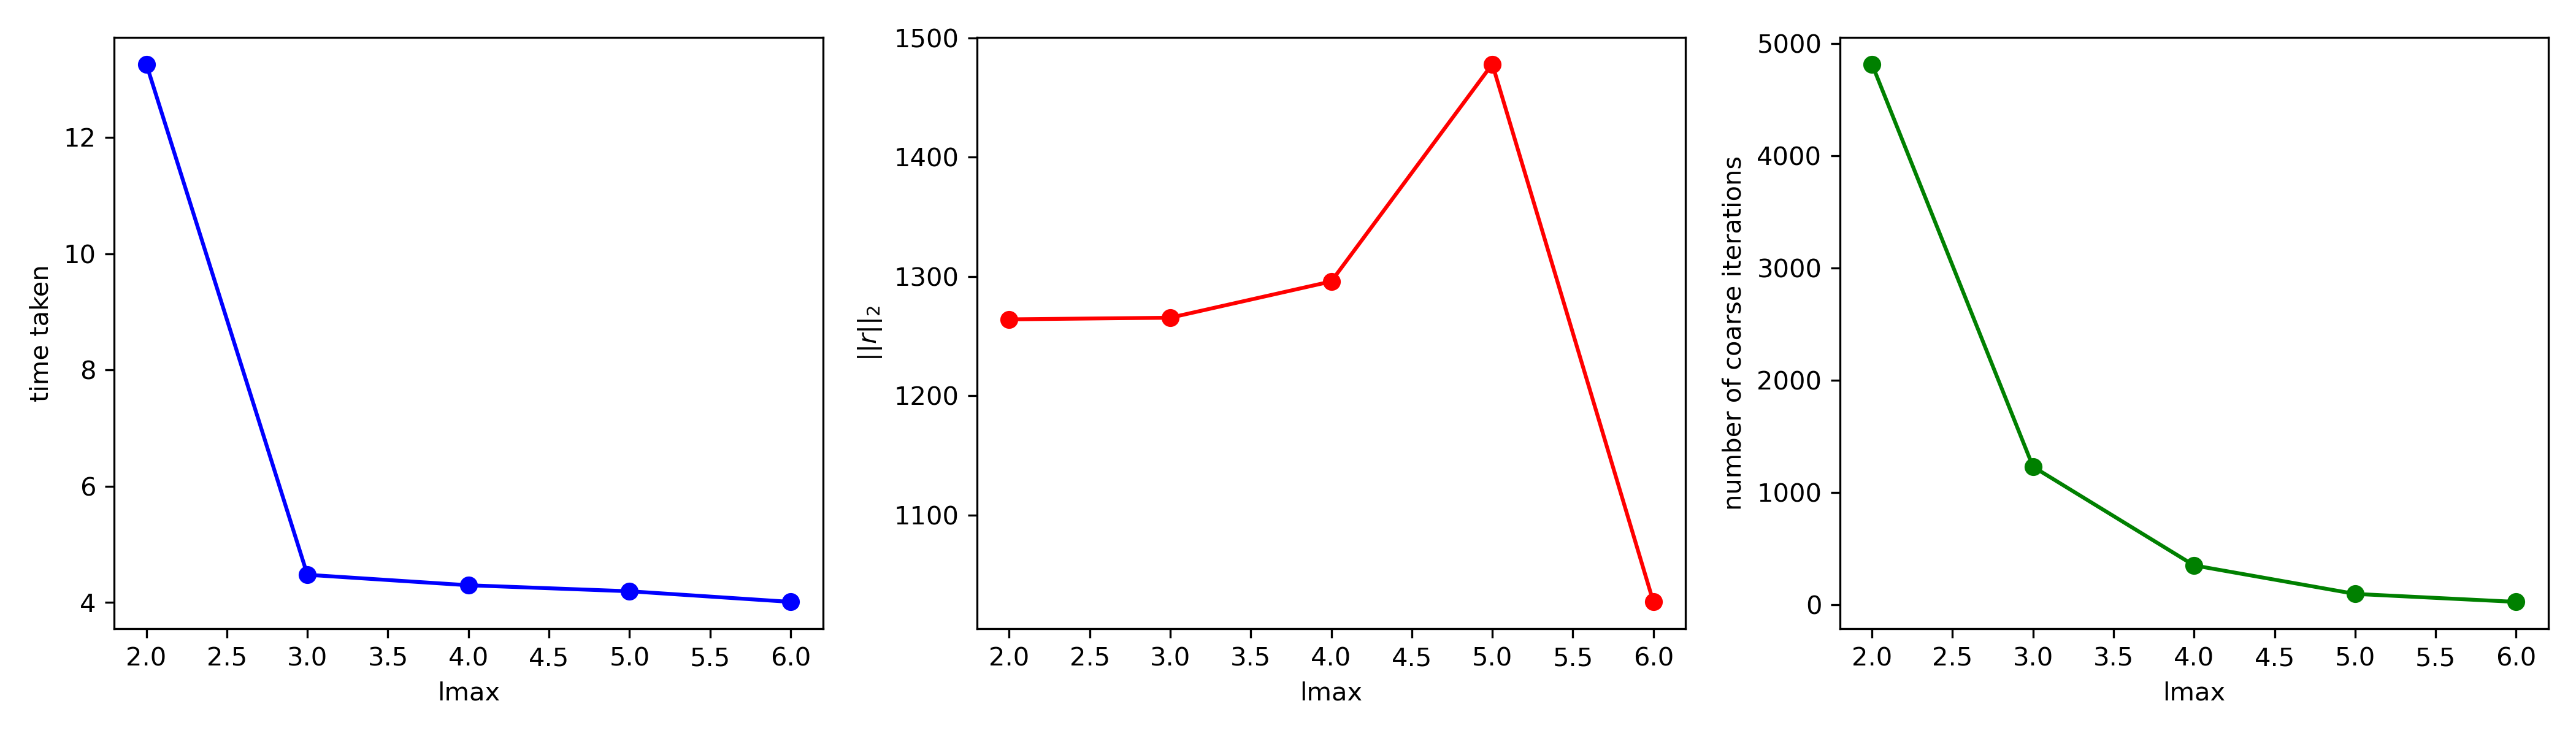
\includegraphics[width=1\linewidth]{./q3_part1.png}
    	%\label{fig:1}
	\end{figure}

\vspace{2cm}


\subsection*{Part 2}
		
	Code run from the file "q3\_part2.c"

	The plots below are only showing $N = 16, 32, 64, 128$. For the value of $N=256$
	I didnt have a machine to use with a sufficent amount of RAM. In the middle plot 
	below you can see that comparing both $lmax$ values the norm of the residual
	changes significanlty and shows us that drastically inscreasing the size numeber
	of levels in $lmax$ has more and more of an impact on the residual. I would assume
	this defficiencly is built in the liner interpolation built into the "prolongation()"
	function. Keeping this in mind and analysing the 
	left and right most plots we can see that $lmax=8$ outpreforms $lmax=2$ in runtime and
	and $lmax=8$ requires a significanly smaller number of iterations to be soled at the
	lowest level.  

		
	\begin{figure}[h!]
	    \centering
    	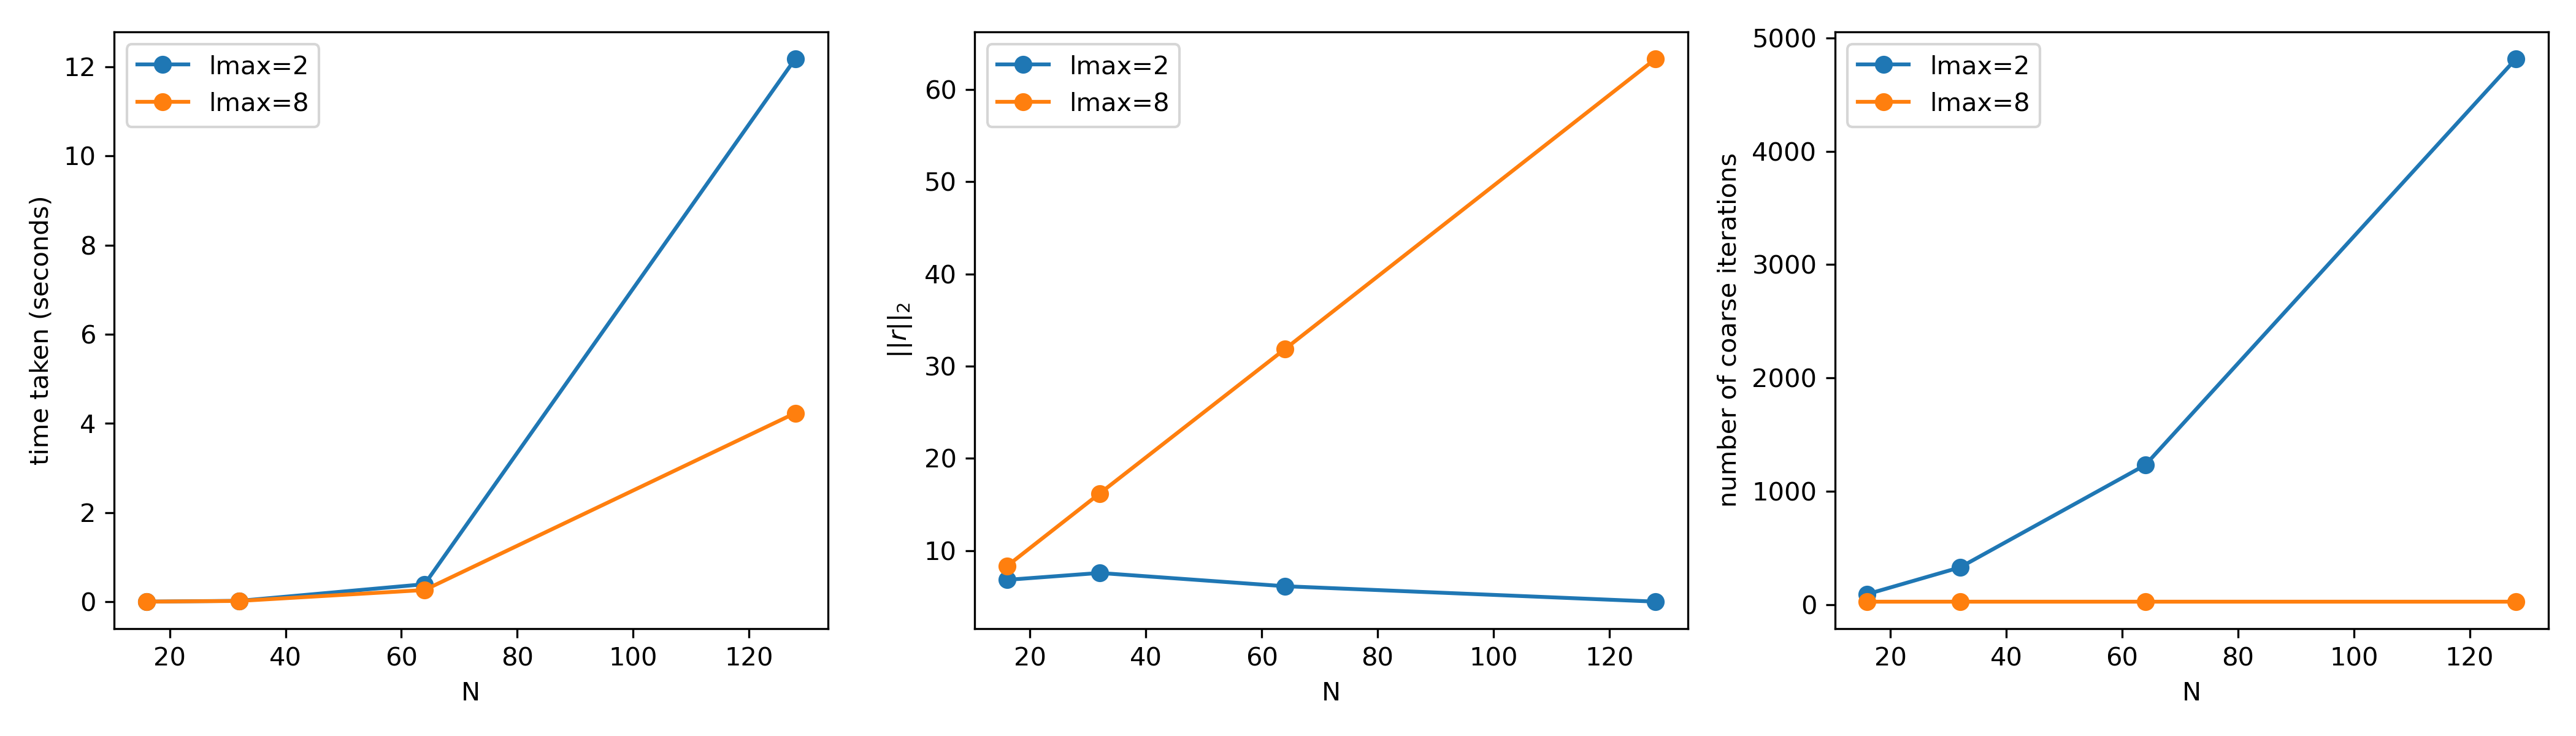
\includegraphics[width=1\linewidth]{./q3_part2.png}
    	%\label{fig:1}
	\end{figure}
	

\bibliographystyle{plain} 
\bibliography{refs} 

\end{document}



